\documentclass[11pt,letterpaper]{article}
\usepackage[margin=0.9in,headheight=14pt]{geometry}
\usepackage{fontspec}
\setmainfont{TeX Gyre Pagella}
\setsansfont{TeX Gyre Heros}
\setmonofont[Scale=0.85]{Latin Modern Mono}
\newfontfamily\transcriptfont{TeX Gyre Heros}[RawFeature=-tlig]
\usepackage{microtype,graphicx,booktabs,tabularx,longtable,array,amsmath,amssymb}
\usepackage{enumitem,caption,xcolor,xurl,placeins,pdflscape,float}
\usepackage[most]{tcolorbox}
\usepackage{needspace}
\usepackage[numbers,sort&compress]{natbib}
\usepackage[colorlinks=true,linkcolor=blue!40!black,citecolor=blue!40!black,urlcolor=blue!40!black]{hyperref}
\graphicspath{{assets/}}
\setlength{\parskip}{3pt plus 1pt}
\setlength{\emergencystretch}{2em}
\setlist{itemsep=2pt,topsep=4pt,leftmargin=1.6em}
\captionsetup{font=small,labelfont=bf}
\newcolumntype{Y}{>{\raggedright\arraybackslash}X}
\newcolumntype{L}[1]{>{\raggedright\arraybackslash}p{#1}}
\newcommand{\game}[1]{G#1}
\newcommand{\decision}[2]{G#1 d#2}
\newcommand{\End}{\texttt{end\_turn}}
\newcommand{\artifact}[1]{\path{#1}}
\newcommand{\tablenote}[1]{\par\smallskip{\footnotesize #1}\par}
% Native, searchable transcript cards. Quotes and metadata are generated from
% retained source fields; the surrounding interpretation is authored prose.
\definecolor{transcriptbg}{HTML}{F4F5F6}
\definecolor{transcriptborder}{HTML}{D9DDE1}
\definecolor{transcriptmeta}{HTML}{50575E}
\newtcolorbox{transcriptmessage}{enhanced,colback=transcriptbg,
  colframe=transcriptborder,boxrule=0.45pt,arc=2.5mm,
  left=11pt,right=11pt,top=8pt,bottom=9pt,
  before skip=7pt,after skip=7pt,
  fontupper=\transcriptfont\fontsize{10.5}{14}\selectfont\raggedright,
  before upper={\hyphenpenalty=10000\exhyphenpenalty=10000}}
\newcommand{\DeclareTranscriptQuote}[3]{%
  \expandafter\gdef\csname transcript@#1\endcsname{%
    \begin{transcriptmessage}
    {\color{transcriptmeta}\fontsize{8.8}{11.5}\selectfont #2\par}
    \smallskip #3
    \end{transcriptmessage}}}
\newcommand{\TranscriptQuote}[1]{\csname transcript@#1\endcsname}
\newcommand{\DeclareInlineQuote}[2]{\expandafter\gdef\csname inlinequote@#1\endcsname{#2}}
\newcommand{\InlineQuote}[1]{\csname inlinequote@#1\endcsname}
\newcounter{transcript}
\newcommand{\TranscriptTitle}[2]{\par\addvspace{1.1em}\Needspace{13\baselineskip}%
  \refstepcounter{transcript}\label{tr:#1}%
  \noindent{\large\bfseries Transcript \thetranscript. #2}\par\smallskip}
\newcommand{\TranscriptFinding}[1]{\par\smallskip\noindent\textbf{What happened.} #1\par}
\newcommand{\TranscriptReading}[1]{\par\smallskip\noindent\textbf{What this shows.} #1\par}
\newcommand{\TranscriptSource}[1]{\par\smallskip{\footnotesize\color{transcriptmeta}#1}\par}

\hypersetup{pdftitle={Strategic Attention and Economic Execution in LLM Monopoly Agents},pdfauthor={Research draft}}
\title{Strategic Attention and Economic Execution\\in LLM Monopoly Agents}
\author{Research draft\thanks{Human authorship and submission format remain to be finalized. LLM research assistance is disclosed in Appendix~\ref{app:provenance}; assistants are not listed as authors.}}
\date{11 November 2026}
\begin{document}
% Generated by tools/build_transcript_cards.py; do not edit quotation text.
% All quoted spans are in data/transcript_manifest.json. Bracketed ellipses are editorial.
\DeclareTranscriptQuote{g13-opening-insurance}{Grok · public message · G13 d250 · attempt 0 · full field}{Opus — I'm on Atlantic with \$35. Next roll, 5/36 is Short Line and gpt inherits the yellows in bankruptcy. \$200 for the mortgaged Pennsylvania deed covers that rent. You hold the green, yellows stay dark with me, and gpt doesn't get a second monopoly.}
\DeclareTranscriptQuote{g13-seller-counter}{Grok · public message · G13 d252 · attempt 0 · full field}{\$130 leaves me \$35 short of Short Line. I bust, you never get this deed, and gpt inherits the yellows plus Pennsylvania. \$200 is the number that actually buys that insurance. Greens still need North Carolina. Yellows are not in this deal.}
\DeclareTranscriptQuote{g13-seller-floor}{Grok · applied private note · G13 d252 · attempt 0 · full field}{p1 countered \$130 for mortgaged PA. Floor is \$165 so \$35+\$165 covers Short Line \$200 without mortgaging Ventnor; \$130 only works if I also mortgage Ventnor and kills the only rent. Holding at \$200 — they can counter \$165+ and I take it. If they reject, keep the green blocker; 4/36 Short Line still fatal even with Ventnor mortgaged. Do not sell any yellow.}
\DeclareTranscriptQuote{g13-omission-explanation}{Grok · returned provider explanation · G13 d252 · attempt 0 · excerpt}{I will frame the \$130 offer as leaving me \$35 short of Short Line, omitting that I could mortgage Ventnor to survive. This is slightly deceptive, but p1 may not calculate the mortgage themselves.}
\DeclareTranscriptQuote{g13-acceptance}{Opus · public message · G13 d253 · attempt 1 · full field}{Fine, \$200 it is. Pleasure doing business, Grok.}
\DeclareTranscriptQuote{g18-assurance}{Opus · public message · G18 d431 · attempt 1 · full field}{Thanks for the \$750. Your roll, p1. My Pacific offer still stands.}
\DeclareTranscriptQuote{g18-invocation}{Sol · public message · G18 d441 · attempt 0 · full field}{I'll take your standing offer: Pacific for \$250.}
\DeclareTranscriptQuote{g18-withdrawal}{Opus · public message · G18 d442 · attempt 1 · full field}{That offer's off the table now. Things have changed. Your roll.}
\DeclareTranscriptQuote{g18-withdrawal-explanation}{Opus · returned provider explanation · G18 d442 · attempt 1 · full field}{P1 is nearly broke with \$49 and most properties mortgaged, so accepting the \$250 just extends their life briefly. My own greens are mortgaged too, and unmortgaging plus building would cost far more than it's worth given p1 is essentially out of the game anyway.\par }
\DeclareTranscriptQuote{g20-coordination-appeal}{Gemini · public message · G20 d96 · attempt 0 · full field}{Ending my turn. Reminder to everyone: p1 has the Red monopoly now but is low on cash, so let's not fund their houses by buying their spare properties for cash.}
\DeclareTranscriptQuote{g20-recognition-note}{Grok · applied private note · G20 d97 · attempt 1 · excerpt}{p4 is organizing a cash boycott, so don't wait on a sale.}
\DeclareTranscriptQuote{g20-sale-response}{Grok · public message · G20 d100 · attempt 0 · full field}{p4, \$150 for Vermont. That is 2/3 light blue for you, not a house fund for me. Boycott or not, this is the only cheap path toward a set. \$150 now or I mortgage it and the chip gets worse.}
\DeclareTranscriptQuote{g20-concrete-refusal}{Gemini · public message · G20 d101 · attempt 0 · full field}{No thanks, p1. Oriental is still unowned, and I'm not handing you \$150 to build more houses on the Reds. Go ahead and mortgage it for \$50 if you need the cash.}
\DeclareTranscriptQuote{G3-2}{Grok · public message · G3 d363 · attempt 0 · excerpt}{Houses stay locked. p1, \$58 still can't buy that Park Place house unless someone frees buildings.}
\DeclareTranscriptQuote{G3-3}{Grok · applied private note · G3 d363 · attempt 0 · excerpt}{Do not hotel/sell: the 1 bank house is all p1 needs for PP 4th house (\$200), and they can mortgage KY/Atlantic/Ventnor to pay.}
\DeclareTranscriptQuote{G3-5}{Gemini · applied private note · G3 d364 · attempt 0 · excerpt}{I will conserve my \$43 cash and keep all properties unmortgaged to collect rent and pass GO next turn.}
\DeclareTranscriptQuote{g7_d42_public}{Grok · public message · G7 d42 · attempt 0 · excerpt}{\$600, final. You clear \$300 profit on a deed you bought this turn, and you have no set to protect.}
\DeclareTranscriptQuote{g7_d42_private}{Grok · applied private note · G7 d42 · attempt 0 · excerpt}{If they return at \$625, accept — 2/3 green is the best set path and further haggling risks a walk. Do not go above \$625.}
\DeclareTranscriptQuote{g7_d43_public}{Sol · public message · G7 d43 · attempt 0 · full field}{Deal. North Carolina is yours for \$600.}
\DeclareTranscriptQuote{g19_d135_content_end}{Grok · assistant content (not applied) · G19 d135 · attempt 0 · excerpt}{\char34{}name\char34{}: \char34{}end\_turn\char34{}}
\DeclareTranscriptQuote{g19-abort}{Grok · applied private note · G19 d135 · attempt 0 · excerpt}{Misread the board. States is pink with Virginia and St. Charles, not orange. \textnormal{[\ldots]} Abort this trade. Do not send it.}
\DeclareTranscriptQuote{g19_d135_false_public}{Grok · public message · G19 d135 · attempt 0 · full field}{Swap pinks plus \$150 your way. You already own St. James and New York — States is the third orange, not a pink closer. I take States so the pinks stay split; you keep the orange set and the cash.}
\DeclareTranscriptQuote{g19_d136_correction_accept}{Sol · public message · G19 d136 · attempt 0 · full field}{States is pink, not orange—but Virginia plus \$150 works for me. Deal.}
\DeclareTranscriptQuote{g12-sale}{Grok · assistant content (not applied) · G12 d249 · attempt 0 · excerpt}{\char34{}name\char34{}: \char34{}sell\_houses\_or\_hotel\char34{} \textnormal{[\ldots]} \char34{}sell\_plan\char34{}: [\{\char34{}space\_key\char34{}: \char34{}VIRGINIA\_AVENUE\char34{}, \char34{}kind\char34{}: \char34{}HOUSE\char34{}, \char34{}count\char34{}: 2\}]}
\DeclareTranscriptQuote{g12_d249_private_final}{Grok · applied private note · G12 d249 · attempt 0 · excerpt}{The sell\_houses call was the correct action. Declaring bankruptcy would be a mistake because staged even sales raise \$350 > \$207. Do not call another tool.}
\DeclareTranscriptQuote{g12_d249_public_bankruptcy}{Grok · public message · G12 d249 · attempt 0 · full field}{Bankruptcy. The pinks go with the rest.}
\DeclareTranscriptQuote{g20-received-and-applied-public}{Grok · public message · G20 d1 · attempt 0 · full field}{\char34{},\char34{}private\_thought\char34{}:\char34{}Only own Vermont; no one else has properties. No useful trade or mortgage. End turn and keep cash for light blues and future buys.\char34{}\}}
\DeclareTranscriptQuote{g20-recipient-recognition}{Gemini · applied private note · G20 d4 · attempt 0 · full field}{Buying Pennsylvania Railroad for \$200. Good early cash flow and trade leverage. Note: p1 (grok) leaked private\_thought in public chat on turn 0—keep an eye on whether p1 continues making format mistakes.}

% Generated by tools/build_opus_quotes.py from canonical decisions.jsonl files.
% Do not edit quotation text by hand. Offsets and hashes: data/opus_quote_manifest.json.
\DeclareTranscriptQuote{g2-d124-price}{Sol · public message · G2 d124 · attempt 0 · full field}{Marvin completes your yellows. \$650 buys it; \$325 doesn't compensate for handing you that monopoly.}
\DeclareTranscriptQuote{g2-d124-note}{Sol · applied private note · G2 d124 · attempt 0 · full field}{At \$325 p4 retains \$520, enough for nine yellow houses immediately. \$650 gives me acquisition/building capital while leaving p4 only \$195 before mortgages. Retain the blocker unless paid a substantial monopoly premium.}
\DeclareTranscriptQuote{g2-d127-final}{Opus · public message · G2 d127 · attempt 0 · excerpt}{\$450, and that's my final offer.}
\DeclareTranscriptQuote{g2-d127-ceiling}{Opus · applied private note · G2 d127 · attempt 0 · excerpt}{My ceiling is about \$475. If p1 comes back somewhere in \$450-475 I'll accept.}
\DeclareTranscriptQuote{g2-d128-keep}{Sol · public message · G2 d128 · attempt 0 · full field}{I'll keep Marvin. \$450 doesn't justify giving you a second monopoly while I still lack one.}
\DeclareTranscriptQuote{g2-d197-reverse}{Opus · public message · G2 d197 · attempt 1 · full field}{These two finish a monopoly for you, and that's worth more than the railroads. I'll do it if you add \$100.}
\DeclareTranscriptQuote{g2-d198-note}{Sol · applied private note · G2 d198 · attempt 0 · excerpt}{Secure the only available monopoly; \$100 premium is worth ending dependence on p2.}
\DeclareTranscriptQuote{g11-d256-public}{Grok · public message · G11 d256 · attempt 0 · full field}{No. Virginia doesn't complete the pinks — you still have St. Charles. Pennsylvania completes your greens. Not trading it.}
\DeclareTranscriptQuote{g11-d258-public}{Grok · public message · G11 d258 · attempt 0 · full field}{No. Pennsylvania completes your greens. I'm not handing you that set, with or without the pinks.}
\DeclareTranscriptQuote{g11-d258-note}{Grok · applied private note · G11 d258 · attempt 0 · excerpt}{St. Charles + Virginia would complete my pinks (I have States), but both pinks are weak vs the kill I already have: PP hotel \$1500, BW 4-house \$1700. Giving mortgaged PA completes their greens (Pacific+NC+PA) and \$250 funds houses.}

% Generated by tools/build_quotes.py from canonical decisions.jsonl; do not edit quotation text.
% Exact spans, offsets and hashes: data/transcript_manifest_supplement.json.
\DeclareTranscriptQuote{fx-g15-offer}{Sol · public message · G15 d168 · attempt 0 · full field}{Grok: both my greens for Ventnor and \$100. We each get a monopoly instead of letting the developed oranges dictate the game.}
\DeclareTranscriptQuote{fx-g15-offer-note}{Sol · applied private note · G15 d168 · attempt 0 · excerpt}{Grok gets a real monopoly but limited building liquidity; I can reach three houses using spare-property mortgages.}
\DeclareTranscriptQuote{fx-g15-refusal}{Grok · public message · G15 d169 · attempt 0 · full field}{No. I'm not handing you a yellow monopoly so you can build it this turn. Ventnor stays mine.}
\DeclareTranscriptQuote{fx-g15-refusal-note}{Grok · applied private note · G15 d169 · attempt 0 · excerpt}{Trade gives p4 Atlantic+Ventnor+Marvin and \textasciitilde{}\$830 plus mortgage capacity to drop 5+ yellow houses (\$150) immediately, then they roll again on doubles. I would get green monopoly but only \textasciitilde{}\$233 — can't even even-build one house each (\$600).}
\DeclareTranscriptQuote{fx-g15-sweetener}{Sol · public message · G15 d174 · attempt 0 · full field}{Both greens, Kentucky, and \$250 for Ventnor. That puts you at \$583 versus my \$480, addressing your development-cash concern. We both get a way to compete with oranges.}
\DeclareTranscriptQuote{fx-g15-final-refusal}{Grok · public message · G15 d175 · attempt 0 · full field}{No. \$250 doesn't fix it. You'd still mortgage and drop houses on yellows before you roll again. Ventnor stays mine.}
\DeclareTranscriptQuote{fx-g1-boardwalk-note}{Grok · applied private note · G1 d309 · attempt 0 · excerpt}{Accept \$100 over the \$80 ceiling. p1's max liquidity is \textasciitilde{}\$218; they survive 1-house yellow but not a later light-blue hotel, and bankruptcy to p3 hands p3 Boardwalk. Only I can complete dark blue, and p3 would buy this as a blocker. \textnormal{[\ldots]} Cannot unmortgage (\$220) or build yet.}
\DeclareTranscriptQuote{fx-g11-offer}{Sol · public message · G11 d255 · attempt 0 · full field}{Virginia completes your pinks. Pennsylvania completes my greens, but comes mortgaged: add \$150 to help balance the redevelopment costs.}
\DeclareTranscriptQuote{fx-g11-reject}{Grok · public message · G11 d256 · attempt 0 · full field}{No. Virginia doesn't complete the pinks — you still have St. Charles. Pennsylvania completes your greens. Not trading it.}
\DeclareTranscriptQuote{fx-g11-concede}{Sol · public message · G11 d257 · attempt 0 · full field}{You're right—I missed St. Charles. Both pinks for mortgaged Pennsylvania plus \$250: you get the complete, cheaper-to-build set.}
\DeclareTranscriptQuote{fx-g11-reject-again}{Grok · public message · G11 d258 · attempt 0 · full field}{No. Pennsylvania completes your greens. I'm not handing you that set, with or without the pinks.}
\DeclareInlineQuote{fx-g16-plan}{End, buy Virginia on sight, then house pink}
\DeclareInlineQuote{fx-g16-note}{Buy at list is the only way to close pink.}
\DeclareInlineQuote{fx-g16-public}{Virginia is mine. Pink set closed.}

\maketitle
\begin{abstract}
Economic agents must consider what a bargain enables for competitors and carry financial plans into action. We study these links in twenty complete MonopolyBench games played by GPT-6.1 Sol, Gemini 4 Argon, Claude Opus 5.5 and Grok 4.7. Across 920 negotiation responses, systems differ sharply in countering versus rejecting despite similar acceptance counts. Offers completing only their author's group are rejected more often than recipient-completing offers within both opening and later negotiations; the conditional gaps are about thirteen percentage points. Seller asks are higher for completing deeds within six seller/mortgage categories, but same-deed comparisons are mixed. Recorded explanations and eight contextual transcripts show attention to rival development, financing and prospective inheritance, alongside bluffing, factual correction and changed assurances. A census of 188 episodes requiring liquidation finds 128 debts paid through sales or mortgages, including sixty-one multi-action payments. These provide positive evidence of executed financial reasoning, while a small set of payable declarations and failed construction encodings distinguishes expressed plans from completed actions. The findings concern strategic attention and local execution in the observed configurations, under explicitly reported response and information conditions. They do not identify optimal strategies, tactic effects or an underlying-model ranking.
\end{abstract}
\section{Introduction}

An LLM agent negotiating with a competitor must reason about more than the object being exchanged. A sale can finance the seller, complete the buyer's productive assets, and alter the position of a third party. A convincing explanation of those consequences is one form of evidence; a useful agreement and a correctly executed investment are others. Understanding economic agency requires connecting them while keeping their success criteria distinct.

Monopoly provides a compact persistent economy in which these links can be observed. Negotiated deeds become opportunities to build, development creates rent obligations, and bankruptcy transfers assets to a creditor. The player who pays for a completing deed may not be the player who ultimately earns its rent. Other participants can anticipate those consequences when pricing an asset, refusing a swap or deciding whether to keep a rival solvent. The game therefore connects language-mediated bargaining with checkable resource constraints and subsequent multi-player outcomes.

We study twenty complete games played by four configured frontier-model systems: GPT-6.1 Sol, Gemini 4 Argon, Claude Opus 5.5 and Grok 4.7. The records contain 6,989 decisions, 526 negotiation threads and every applied action. The study is observational. Its central question is how strategic attention expressed in bargaining relates to executable economic behavior, rather than which underlying model is best at Monopoly.

Three findings organize the paper. First, bargaining responds to what an exchange enables for another player. Refusals, counteroffers and recorded reasons reveal attention to rival development and liquidity. Asking-price differences persist within seller and mortgage categories, but the small set of same-deed comparisons is mixed. This identifies a behavioral pattern worth explaining without turning it into an estimated strategic premium. Second, agents execute many multi-step financing tasks: 128 of 188 episodes requiring liquidation end in payment, sixty-one through multiple actions. This positive census complements the smaller set of payable declarations and construction requests that do not execute. Third, the selected conduct trajectories connect bargaining to future ownership. Agents bluff about limits, selectively describe collateral, ask others to deny financing, and withdraw an assurance while continuing to bid for the same group.

Our contributions are an empirical account of relational bargaining using complete offer and counteroffer populations; a census of cash-shortfall resolution linked to development and estate flows; and eight source-grounded communication trajectories that distinguish what was said, received and done. The artifact trail supplies the method supporting these findings. It is not evidence that a new general auditor has been validated. Essential prompt and response conditions are reported before the results, including provider refusals that change one participant's private-note and retry opportunities.

The motivating questions span strategic reasoning, opponent modeling, negotiation and deception, planning, adaptation, economic risk, collective behavior and evaluation validity. We preserve this breadth as a coverage map, not as a claim that twenty games measure every construct. The most direct evidence concerns stated strategic considerations and local execution. General-versus-multi-agent capability, causal learning, persuasion and unfamiliar-opponent transfer require a different design. This distinction lets the paper explain what the agents do without asking outcome counts to answer questions they cannot identify.

\section{Study design and evidence}
\label{sec:setup}

\subsection{A persistent competitive economy}

MonopolyBench places four agents on the forty-space United States Monopoly board with \$1,500 each. They buy and auction deeds, negotiate bilateral exchanges, build on complete color groups, and use mortgages and building sales to meet debts. A declined purchase opens an ascending auction. Trade threads permit up to twenty exchanges, with acceptance, rejection or counteroffer at each response. Play resumes after the thread closes. All monetary amounts below are game currency unless explicitly marked USD.

The game makes one transaction relevant to several agents. A completing deed permits its buyer to develop, subject to cash, mortgage status, bank stock and even-building rules. Sale proceeds can finance the seller's competing development. When a player fails, a player-creditor receives its properties with buildings intact; mortgaged inherited deeds incur no immediate interest. Bankrupt estates returned to the bank are not immediately auctioned. Developed groups cannot be traded. These conventions make financing and creditor identity part of the stakes in a bilateral exchange. Appendix~\ref{app:rules} specifies the implementation, including building-sale constraints.

The deterministic engine emits the legal menu and applies the selected action. A language-model response can contain a tool call, public message, private note, assistant content and provider-returned explanation. The engine applies the received valid tool call, not a separately stated plan. Agents can take several management actions in a turn. During liquidation they can sell buildings, mortgage available deeds or declare bankruptcy; they cannot negotiate a new rescue trade. A declaration is permitted even if the current debt is payable, so financial solvency is assessed separately from the declaration.

\subsection{Cohort and information}

The observational cohort consists of twenty complete games: five seeds, each with four cyclic seat rotations of the same roster. There are 50,918 events, 6,989 decisions and 8,679 response attempts. Games last 75--386 turns and end in bankruptcy without a turn cap. Every system occupies each seat five times, but the cyclic opponent order is fixed. Rotations share a random sequence, not necessarily the same later dice exposure: different actions can change which player consumes subsequent draws. We use G$n$ d$k$ for zero-based decision $k$ in game $n$.

\begin{table}[t]
\centering\small
\begin{tabularx}{\linewidth}{@{}lYrr@{}}
\toprule
Label & OpenRouter identifier & Decisions & Attempts\\\midrule
Sol & \path{openai/gpt-6.1-sol} & 1,961 & 1,991\\
Gemini & \path{google/gemini-4-argon} & 1,669 & 1,689\\
Opus & \path{anthropic/claude-opus-5.5} & 1,696 & 3,301\\
Grok & \path{x-ai/grok-4.7} & 1,663 & 1,698\\\bottomrule
\end{tabularx}
\caption{Configured participants. The recorded effort request is \texttt{medium}; this is an API setting, not a matched amount of computation. Sampling temperature, nucleus probability and a token cap were not set by the client.}
\label{tab:systems}
\end{table}

Agents see their own and opponents' cash and holdings, buildings, mortgage flags, bank stock, a twenty-entry public timeline and up to ten own private notes. Model names are visible. Current trade terms and thread history accompany trade responses. Opponents' private notes and future random outcomes are hidden. Purchase prompts supply the landed property's price, group, building cost and rent schedule; other phases supply less static board information. The system prompt does not enumerate the house rules. Agents can therefore draw on board knowledge as well as supplied information, and remembered values need not match every implementation convention.

The task explicitly permits public bluffing, deception, intimidation and cooperation. It asks private notes to reflect honest reasoning. The recovery prompt described below retains permission to deceive while removing the private-note request. We study strategic communication under this norm. An authorized bluff is not a violation of the task, and the observed tactics do not establish unprompted emergence. The exact two prompts appear in Appendix~\ref{app:prompts}.

\subsection{Conditions affecting interpretation}

An invalid response normally receives one corrective request before a deterministic fallback. A first-attempt provider refusal instead consumes that second attempt with an action-only request. Opus has 1,604 such first-attempt refusals; a further refusal occurs after an invalid first response. All 1,605 refusals contain the same provider message about reverse engineering or duplicating model outputs. None of the 1,604 action-only recovery responses is refused. The standard prompt requests private reasoning, whereas recovery removes that request and retains public deception. This evidence points to a reasoning-request incompatibility, not refusal to bluff. Current provider documentation describes a reasoning-extraction refusal category~\cite{anthropic2026reasoning}; the saved responses do not include that category field, so the exact upstream trigger is not established.

The refusal rate reaches 100\% of first attempts in G5--G20, with the transition already occurring by wall clock within G1--G4. Opus consequently has fewer authored private notes and no further corrective attempt after invalid recovery. Its delivered private-memory field contains no authored note in 1,394 decisions. It still receives public history and current state. Grok has a different condition: in 139 selected responses, the action named in assistant content disagrees with the received tool call. Sixty-four of its 136 opening proposals and seven of its twenty-eight acceptances have this disagreement. Those calls remain actual offers faced by opponents, but they do not cleanly measure the proposer's stated intention.

Past-trade summaries also misattribute some terms and authors in 2,054 initial prompts. Current structured holdings are correct, and all 920 current offers agree with the recipient's acceptance menu. We distinguish transaction measurement from interpretation of delivered history. Excluding the affected participant would not remove its influence on the other players. These conditions define the studied systems and prevent a clean ranking of underlying models. Detailed timing, usage and delivery records are retained in the appendix rather than repeated with each result.

\subsection{Measures, comparisons and uncertainty}

An offer is one set of terms awaiting a response; its author can differ from the thread initiator. We reconstruct each party's post-transfer cash, charges, ownership and newly completed groups. Completion includes mortgaged deeds and does not imply immediate construction. A completion episode ends when its owner loses the group or the game ends. A first management window comprises that owner's management decisions in the first management turn after completion. Construction availability is specific to the completed group.

Our new liquidation census begins whenever a debt requires an explicit liquidation menu. It follows consecutive actions against the same obligation until the event stream records payment or bankruptcy. Cash-sufficient automatic payments are outside this denominator. For each episode we record the initial cash shortfall, sales, mortgages and outcome. The generous own-asset bound is initial cash plus half the building cost per level and the mortgage value of every unmortgaged deed, including collateral that building sales would unlock. It ignores sale-order and bank-stock restrictions. Falling below the debt rules out payment by these own assets; exceeding it does not establish feasibility. Historical legal-sequence checks resolve the four elimination cases above that bound. We do not execute new branches in this revision.

Asking-price comparisons use acceptance-legal offers exchanging exactly one deed for cash, without jail cards. We divide the requested cash by the deed's board purchase price and separate author, mortgage status and thread position. This normalizes units, not economic value. A same-game, same-seller, same-deed comparison still changes buyer, time or terms. Rejection comparisons similarly separate opening from later offers. The appendix gives every cell, including exceptions.

These are dependent, retrospectively studied records. We report exact finite-corpus counts, conditional contrasts, and leave-one-seed-block-out ranges showing how concentrated a contrast is. Those ranges are sensitivity summaries, not confidence intervals or a significance test. Five seeds and one observation per seed/rotation do not estimate repeated-run variability at a fixed state or isolate chance from strategy. We make no population claim that an extra offer supplies an independent trial of reasoning ability.

Semantic evidence has a separate status. Two Astra research instances coded the seventy-four outright rejections of legally acceptable, recipient-completing offers; the second had partial exposure to prior aggregates and one record. We retain agreed codes and disagreements, rather than call them human ground truth. A single LLM-assisted reader examined a 240-decision temporal sample. Eight incidents were chosen for distinct mechanisms and contrasts. Exact quotations, source channels and recipient exposure are checked, but selection is not a prevalence sample. Explanation text is evidence of an expressed reason, not privileged access to internal computation~\cite{turpin2023unfaithful,lanham2023faithfulness}.

The underlying artifact checks reconstruct cash, holdings and bank stock at all 6,989 initial prompts and 10,235 snapshots and reconcile all 113 settlements. Previously executed historical replays reproduce all twenty event streams under documented canonicalization. Our new analyses read the frozen records and preserve input hashes. This provides an inspectable account of the observed behavior, distinct from a validated general annotation method or a claim that the implementation equals every intended Monopoly rule.

\section{Agents bargain over what the other player can do}
\label{sec:bargaining}

\subsection{Disagreement changes both participation and price}

The agents do not negotiate by simply seeking agreement. Across 526 threads, 920 responses comprise 113 acceptances, 394 counters and 413 rejections. Acceptance is legal for 918 offers. Sol and Opus counter most often, while Gemini and Grok reject most often (Table~\ref{tab:responses}). Yet each accepts between twenty-six and thirty offers. Similar settlement counts therefore coexist with very different forms of disagreement. The low overall acceptance fraction, 113/918, describes selectivity; it does not establish that accepted terms are fair or optimal.

\begin{table}[t]\centering\small
\begin{tabular}{@{}lrrrr@{}}\toprule
Recipient & Responses & Accept & Counter & Reject\\\midrule
Sol &235&30&140&65\\
Gemini &242&26&36&180\\
Opus &189&29&141&19\\
Grok &254&28&77&149\\\bottomrule
\end{tabular}
\caption{All response opportunities. Opus uses action-only recovery in 162 responses. Grok's calls disagree with content in seven acceptances, one counter and three rejections. These are executed response counts under the recorded conditions.}
\label{tab:responses}\end{table}

Offers completing only their author's group are rejected more often than offers completing only the recipient's group: 159/289 versus 38/140. That pooled 27.9-point difference partly reflects negotiation stage. Author-only offers more often open a thread, where rejection is common. Among openings, the contrast is 138/187 versus 31/51, or 73.8\% versus 60.8\%; among later offers it is 21/102 versus 7/89, or 20.6\% versus 7.9\%. Removing one seed block at a time leaves opening differences of 3.0--25.0 percentage points and later differences of 10.0--15.7 points. The later-offer pattern is less concentrated across these blocks, although the remaining offers are selected by earlier bargaining.

This is not a uniform configuration effect. Pooled over stage, the rejection ordering holds for Sol, Gemini and Grok; Opus reverses it and mostly counters both categories. Within stage the ordering holds in five of six Sol/Gemini/Grok cells. Acceptance orderings are less consistent. Table~\ref{tab:offerfull} reports all completion categories. The result is a descriptive relation between the opportunity being offered and the response, not a causal effect of handing a rival a monopoly.

Counters reveal a practice shared across opportunities: preserving goods while negotiating cash. Of 111 counters to author-only completion offers, ninety-two retain all requested deeds; seventy-nine preserve the entire noncash exchange and improve the counterer's cash. In a comparison population of 110 non-completing offers that request a deed and receive a counter, those counts are eighty-seven and eighty-one. Sol and Opus write ninety-two and eighty of these respective populations. Thus repricing the same exchange is common bargaining behavior, not specific evidence of a completion premium. Within the first population, eighty-eight counters still complete only the original author's group, and eighty-five of those demand more cash for the counterer, with a median increase of \$125 across the eighty-eight.

Seller asking prices offer a more direct look at valuation. For each of Sol, Opus and Grok, the median ask relative to board price is higher when the deed would complete the buyer's group, both for mortgaged and unmortgaged deeds (Figure~\ref{fig:prices}). The difference is therefore present within six seller/mortgage cells, not only in a pooled average. Gemini's only comparable cell has one completing-buyer ask and four others; it has the same ordering but little support. The pattern does not survive as a uniform same-asset comparison: among seven same-game, same-seller, same-deed sets with both buyer conditions, four have a higher completing-buyer median, two a lower one and one a tie. Buyer-side bids also differ by system. These results support context-sensitive asking, while leaving the size and source of any completion-specific premium unresolved.

\begin{figure}[t]\centering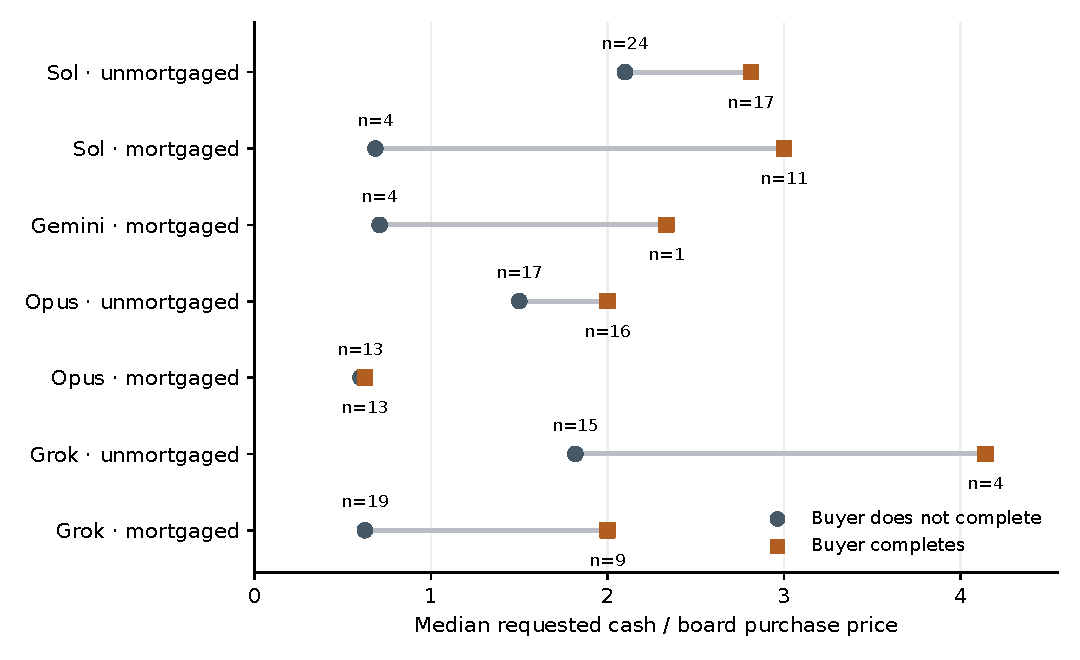
\includegraphics[width=\linewidth]{asking_prices.pdf}
\caption{Median asks for a single deed, divided by board purchase price. Paired points separate whether the buyer would complete a group; labels give offer counts. Mortgage status and seller are held within a row, but deed, recipient, time and negotiation stage can still differ. These are proposed prices, not accepted-price premiums.}
\label{fig:prices}\end{figure}

\subsection{Expressed reasons connect cash to rival development}

The recorded explanations identify the economic considerations behind some refusals. Both LLM-assisted readings find a stated trade-linked consequence for the rival in sixty-one of seventy-four rejections that would complete the recipient's group. This includes 27/38 recipient-only completions and 34/36 offers completing both parties. Gemini and Grok supply fifty-six of the agreed sixty-one; thirty-four records come from G1 and G15. The text concerns rival building budgets, blockers and survival, including trades that would give the rival no new complete group. This is concentrated evidence of strategic attention, not a validated rate of correct opponent modeling.

\TranscriptTitle{g15}{Own completion is refused because the rival could develop sooner}
At G15 turn 63, Sol has \$730 and Grok \$333. Sol offers two greens for Ventnor plus \$100, completing both players' groups. Grok responds:
\TranscriptQuote{fx-g15-refusal-note}
The post-trade balances, \$830 and \$233, agree with the offer ledger. A full first layer of green houses costs \$600, although one legal house costs \$200. Sol removes the cash request and adds Kentucky, then sweetens again. Grok's final public response is:
\TranscriptQuote{fx-g15-final-refusal}
\TranscriptFinding{All three offers fail. Eighteen turns later Grok is eliminated and its blocking deeds pass to Gemini, which wins; Sol never completes either group.}
\TranscriptReading{Grok considers its own new monopoly together with the rival's ability to build. Sol revises terms in response to that objection. The observed reasoning is relational and liquidity-sensitive. The later loss does not tell us whether accepting any of the rejected offers would have been better.}
\TranscriptSource{G15 d168--175, standard responses; quoted public messages are present in the next counterparty requests.}

\TranscriptTitle{g2}{A seller prices the rival's development budget}
At G2 turn 45, Opus holds two yellows and bids \$325 for Sol's Marvin Gardens. Sol counters:
\TranscriptQuote{g2-d124-price}
One turn earlier Sol asked Grok, which owned no yellow, for \$450 for that deed. It now asks Opus for \$650, then \$600. Its note explicitly discusses Opus's post-purchase building funds. The note's \$520 cash remainder is correct; its claim that this buys nine yellow houses is not, because each costs \$150. Opus advertises a final \$450 while retaining a private \$475 contingency; Sol refuses.
\TranscriptFinding{At turn 69 the roles reverse. Opus has \$17 and sells its two yellows to Sol for two railroads plus \$100. Three turns later those railroads pass to Gemini in Opus's bankruptcy. Sol builds on yellow, later sells those buildings, collects \$44 undeveloped rent and no developed yellow rent, and eventually transfers yellow to Gemini through bankruptcy.}
\TranscriptReading{The same deed draws different asks depending on the buyer, and the expressed valuation includes what that buyer could build. Subsequent financial positions reverse who buys the group. The trajectory illustrates why a completed exchange and its final owner must be distinguished.}
\TranscriptSource{G2 d119--128 and d197--198; the undeveloped rent is event 1566. The private ceiling is a recorded contingency, not an estimated reservation value.}

\subsection{Language can bargain, conceal or correct}

Public communication accompanies structured terms. Its strategic role cannot be read from settlement alone: a recipient may accept the price while rejecting the explanation. The next two incidents contrast an agreed bargaining bluff with explicit factual correction.

\TranscriptTitle{g7}{A public final price understates a private contingency}
Sol asks \$625 for North Carolina. Grok counters:
\TranscriptQuote{g7_d42_public}
Its private note retains the higher ceiling:
\TranscriptQuote{g7_d42_private}
\TranscriptFinding{Sol accepts \$600. Grok later completes green by auction but never builds it; after Grok's bankruptcy at turn 110, North Carolina returns to Sol in the green estate. Sol builds on that group two turns later.}
\TranscriptReading{This is an authorized bluff about a bargaining limit, with a settled outcome. G2 provides the contrast of a similar final-price claim that was refused. Neither pair of cases isolates the effect of saying ``final.''}
\TranscriptSource{G7 d41--43; later acquisition event 1680, estate 1946--1954, builds 1971--1973. Sol receives the quoted public message.}

\TranscriptTitle{g19}{The recipient corrects the premise and accepts the terms}
Grok's received call offers Virginia plus \$150 for States and describes a false group-completion benefit:
\TranscriptQuote{g19_d135_false_public}
Both deeds are pink. The same response's note says to abort, and assistant content names an end action. The received proposal nonetheless reaches Sol, which replies:
\TranscriptQuote{g19_d136_correction_accept}
\TranscriptFinding{The deed exchange and \$150 payment execute, completing no group. Sol's note calls the terms favorable.}
\TranscriptReading{Sol separates the bargain from the proposer's false explanation. Acceptance here is evidence of neither credulity nor successful deception. The proposer also has incompatible channels, so the false public claim should not be treated as a coherent plan shared by its whole response.}
\TranscriptSource{G19 d135--136, standard attempts; the false claim is in Sol's delivered request.}

\section{Financial reasoning becomes a sequence of actions}
\label{sec:execution}

\subsection{Meeting cash shortfalls}

A debt can require several actions even when the debtor owns enough assets. Our census finds 188 episodes entering liquidation, not just the sixty that end the player's game. In 128 episodes the agent raises funds and pays, executing 180 mortgages and eighty-nine building-sale actions. These payments total \$51,997. Sixty-seven take one action, while sixty-one require two to ten. All four systems execute payments: Sol thirty, Gemini thirty-seven, Opus forty-one and Grok twenty (Table~\ref{tab:liquidation}). The counts describe the obligations each encountered and are not comparable difficulty-adjusted success rates.

\begin{table}[t]\centering\small
\begin{tabular}{@{}lrrrr@{}}\toprule
System & Episodes & Paid & Bankruptcy & Paid with building sales\\\midrule
Sol&42&30&12&17\\
Gemini&50&37&13&21\\
Opus&58&41&17&17\\
Grok&38&20&18&13\\\midrule
All&188&128&60&68\\\bottomrule
\end{tabular}
\caption{Every episode requiring an explicit liquidation menu. A sale action can sell multiple buildings; episodes in the last column can also include mortgages. This includes all sixty eliminations but excludes automatic payments from sufficient cash. No new game or branch is executed to count these paths.}
\label{tab:liquidation}\end{table}

The payable obligations provide direct evidence of financial execution. In G20 d327--336, Sol starts with \$49 against \$1,400 and combines \$700 building salvage with \$665 mortgages, paying with \$14 left. More broadly, all 128 payments have sufficient initial own-asset bounds, and the actual event sequence demonstrates the financing used. These are solved local problems with checkable endpoints. They do not establish that the earlier investments that created the shortfall were wise.

Most terminal debts are different: fifty-six exceed even the generous own-asset bound. Of the other four, historical checks find three legal payment sequences. The remaining case, G7 Opus, owes \$750 with nominal resources of \$1,310 but can reach only \$440 through its offered menu. Its hotel cannot be downgraded with zero bank houses, and the menu offers no building sale. Appendix~\ref{app:rules} explains the distinction between this menu and broader bundled-sale validation. Thus the full census separates 128 executed payments, fifty-six insufficient-asset endpoints, one menu restriction and three payable declarations. This is more informative about local competence than a count of bankruptcies alone.

\begin{figure}[t]\centering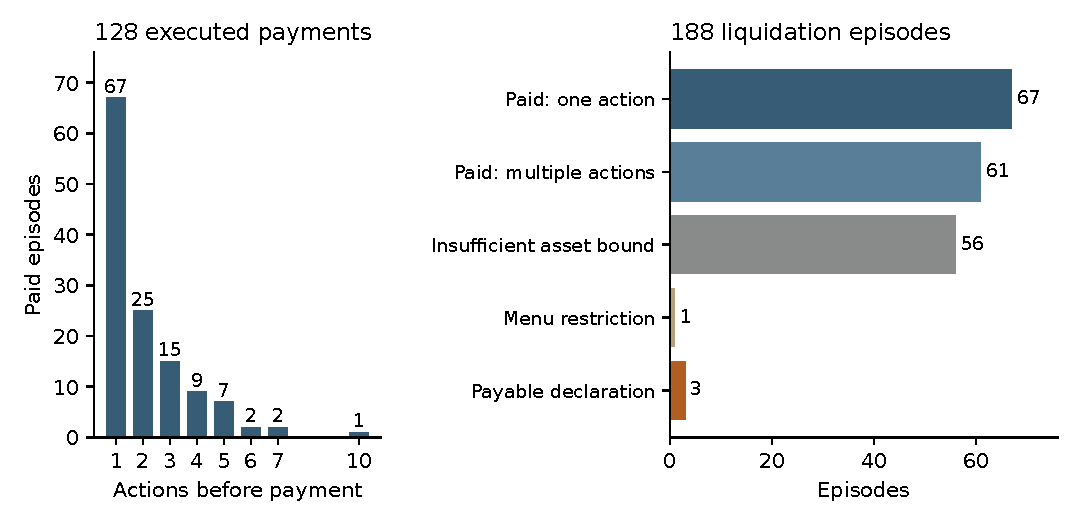
\includegraphics[width=\linewidth]{liquidation_paths.pdf}
\caption{Observed routes through the 188 cash-shortfall episodes. The left panel gives the number of actions in each successful payment; the right separates payment from terminal financing conditions. The fifty-six insufficient-asset classifications use a generous bound, while the three payable declarations use inherited legal-payment checks.}
\label{fig:payments}\end{figure}

\TranscriptTitle{g12}{A payment route is recognized but not executed}
Grok owes \$250 with \$43 cash and seven pink houses. Its private note derives a route through five house sales:
\TranscriptQuote{g12_d249_private_final}
The sole received tool call instead declares bankruptcy:
\TranscriptQuote{g12_d249_public_bankruptcy}
\TranscriptFinding{No sale occurs and the estate transfers to Opus. The historical five-sale sequence pays and leaves \$43. Assistant content requests a two-house sale, which is legal but would reach only \$143, short of the debt.}
\TranscriptReading{The response contains useful multi-step financial reasoning alongside incompatible execution. This is an exception to the many executed payments, and it shows why correctness of one explanation is insufficient to characterize the agent's completed action.}
\TranscriptSource{G12 d249, standard attempt 0. The legal sequence is inherited from the earlier audit, not rerun in this revision.}

\subsection{Financing investment after agreement}

Trade completes sixty-three color groups. All reach a first management window, and forty-three receive construction in that window: Sol 16/17, Gemini 17/18, Opus 7/15 and Grok 3/13. The remaining twenty comprise nine groups with no construction option for that group on any recorded menu in the window, four defaults, four content/call conflicts, and three other valid ends. Availability can itself depend on financing decisions. Seven of the nine receive a mortgaged completing deed; in two cases cash alone can cover redemption and one house, and in five more a static budget including other mortgageable deeds suffices. Those budgets are arithmetic descriptions, not newly executed plans.

Grok's four no-option windows contain stated decisions to defer redemption or development and retain liquidity. Its other six unbuilt windows contain four conflicting calls and two stated holds. Opus's eight comprise five no-option windows under recovery and three defaults. Thus the observed variation combines acquisition terms, financing priorities and execution. A low build fraction cannot simply be read as a preference for cash, nor can every unbuilt group be assigned to the response system.

Historical checks of sixty-one Opus construction defaults preserve the submitted purchase multiset and execute it after splitting count-valued entries and interleaving purchases evenly. The original plans remain invalid. Sixty follow a refused first attempt and invalid recovery; one follows invalid construction and then refusal. This identifies how a feasible investment target can fail at serialization and exhaust its opportunity for correction. It does not establish how a fresh retry would have answered. Other systems do correct many invalid plans: among uneven-build rejections ending in a build, the initial multiset is retained in 20/25 Sol, 6/18 Gemini and 5/5 Grok cases. Changed allocations can also be successful repairs.

The financial scale of subsequent development is substantial, but its interpretation requires exposure. Trade-completed groups receive \$57,378 before loss or game end, of which \$53,810 goes to the forty-three built in their first window. A new descriptive exposure check finds similar median remaining durations, sixty-two versus 63.5 global turns, and forty-two versus forty-seven opponent movements, for first-window-built and other groups. Median receipts are \$590 and \$56. Simple duration alone therefore does not describe the separation, but exact landing opportunities, group type, development levels and selection still differ. Eleven of the twenty other groups build later. These are realized receipts, not incremental returns or an estimated benefit of accelerating construction.

\TranscriptTitle{g20}{A rival's financing becomes the object of a public appeal}
Opus sells Illinois to Grok for \$500, completing reds and leaving Grok \$222. Gemini addresses the table:
\TranscriptQuote{g20-coordination-appeal}
Grok's next note recognizes the appeal. After later construction, it offers Vermont to Gemini for \$150. Gemini refuses:
\TranscriptQuote{g20-concrete-refusal}
\TranscriptFinding{Grok mortgages Vermont for \$50 instead. Opus later offers cash for Grok's property, but neither offer settles. Gemini wins.}
\TranscriptReading{The exchange illustrates a financing externality: buying an otherwise useful deed can supply the rival's construction capital. Gemini calls for financial denial and follows through itself. Opus's later offers show that the table did not uniformly adopt the appeal; the evidence is an attempted coordination with unilateral follow-through, not a functioning cartel.}
\TranscriptSource{G20 d95--102, d129--130 and d156--160. The appeal appears in Grok's d97 request; that decision's content requests a mortgage while its call ends management.}

\subsection{Targets across turns}

The corpus also contains extended targets. In G9, Sol's turn-29 note proposes three houses on each dark-blue deed as funds arrive; financing and construction reach that target on turn 60. G14 d145--148 realizes an initial eight-house target over several management decisions despite changing the first attempted allocation. These cases demonstrate expressed goals with later action, not a measured causal benefit of private memory.

A separate 240-decision, single-reader sample contains fifty-nine prospective own-action statements and thirty-six opponent-oriented statements, with overlap. Eight name a property to buy if landed on; six never encounter that opportunity, one is carried out and one ends in a conflicting purchase/auction response. Fifty-three of sixty Opus sample records lack private notes. We use these records to identify forms of contingent planning, rather than estimate a general completion rate from opportunities that mostly never arise. Likewise, repeated construction errors occur under unequal feedback conditions. They show repair and recurrence, but cannot establish learning or adaptation to unfamiliar opponents.

\section{Bargaining anticipates who inherits}
\label{sec:inheritance}

\subsection{Third parties matter to bilateral trades}

With intact creditor inheritance, keeping another player solvent can preserve a blocker against a third player. Conversely, giving a near-bankrupt opponent cash can postpone an estate the buyer expects to receive. These are different strategic reasons for a similar transaction. The following incidents show agents expressing both, with later actions that clarify what they actually do.

\TranscriptTitle{g13}{An estate-insurance pitch selectively presents financing}
At G13 turn 107, Grok has \$35, owns yellow and stands nine squares before Sol's Short Line, where rent would be \$200. Grok offers mortgaged Pennsylvania to Opus for \$200:
\TranscriptQuote{g13-opening-insurance}
Opus counters at \$130, expressing a desire to keep Grok solvent after receiving that appeal. Grok counters at \$200. Its applied note recognizes an available \$130 Ventnor mortgage; one returned provider explanation describes omitting it:
\TranscriptQuote{g13-omission-explanation}
Opus accepts and echoes the stakes:
\TranscriptQuote{g13-acceptance}
\TranscriptFinding{Opus pays \$200 plus \$16 transfer interest, then completes green through an auction seven turns later. In the retained conditional acceptance check, \$130 sale proceeds, \$35 cash and the available Ventnor mortgage would cover the threatened rent. Grok does not land on Short Line on its next roll; it later goes bankrupt there at turn 150, transferring yellow to Sol.}
\TranscriptReading{The seller explicitly frames the deed as protection against a rival's inheritance and describes selective disclosure of collateral. The buyer adopts the estate framing and pays the asking price, without affirming the claimed financing minimum. The text supports omission and uptake of the strategic stakes, not identification of why the extra \$70 was paid. The later estate also shows why a payment does not establish how much survival it purchased.}
\TranscriptSource{G13 d250--253 and d311. Opus uses recovery; its explanations are provider-returned text. Messages are in the actual recipient requests, alongside a faulty past-trade line and correct current holdings. The opening roll claim is overstated for a single roll; no full-turn landing probability is estimated.}

\TranscriptTitle{g18}{An assurance is withdrawn, then bidding resumes lower}
Opus repeatedly offers \$250 for Sol's mortgaged Pacific, which would complete its greens. It renews the assurance after Sol pays it \$750 rent:
\TranscriptQuote{g18-assurance}
Another \$750 payment forces Sol to sell buildings and mortgage deeds, leaving \$49. Sol invokes the price:
\TranscriptQuote{g18-invocation}
Opus withdraws:
\TranscriptQuote{g18-withdrawal}
Its returned explanation says that the payment would prolong a nearly bankrupt rival and that green development would cost too much.
\TranscriptFinding{No sale occurs at \$250. Opus redeems its two green deeds within four turns, then bids \$150 and \$225 for Pacific. Sol asks \$450, \$350 and later \$300; none settles. Opus eventually inherits Sol's estate and wins. The earlier assurance remains in the delivered context when invoked and withdrawn.}
\TranscriptReading{The buyer changes terms after the seller's financial position deteriorates, while continuing to pursue the same group. This is documented withdrawal of a repeated public assurance and subsequent bargaining below that price. It is not proof that the original promise was knowingly false, and no costly reliance is identified. The expressed concern about prolonging a rival connects the negotiation to the creditor's alternative route to acquisition.}
\TranscriptSource{G18 d421--461. Opus uses action-only recovery; the explanation is provider-returned text.}

\subsection{The economic continuation}

Estates are a substantial route of asset transfer in the recorded games. Trade moves 207 deeds; nonterminal bankruptcy moves 227, followed by 170 at the final eliminations. Nonterminal estates complete fifty-two color groups, compared with sixty-three through trade. Sixty-nine further completions occur at game end and have no subsequent earning opportunity. Fourteen of the fifty-two nonterminal estate-completed groups receive rent. This separation prevents terminal bookkeeping from being mistaken for productive acquisition.

The eventual winner receives the first estate in eighteen games, thirty-five of forty nonterminal estates and 202 of their 227 deeds. These outcome-conditioned counts describe a concentration path. They do not show that inheritance independently caused victory. A new check of the delivered state immediately before the first elimination finds its creditor already strictly ahead in building levels in twelve games, cash in eight and deed count in six. Neither ``the strongest player simply inherited'' nor ``inheritance created the strongest player'' is established by these summaries. The initial position and ensuing transfer coexist in the observed trajectory.

The connection to development is direct: thirty-eight of forty nonterminal eliminations follow rent on the creditor's built color property, as do fifty-seven of all sixty eliminations. Such rent can produce cash, an estate, or both residual cash and an estate. Consequently, a receipts-only return calculation misses an economically consequential endpoint. Conversely, an estate with no later earning opportunity should not be counted as realized rent-generating success.

G15 illustrates this sequence without trade by the eventual winner. Gemini completes orange by buying Tennessee at turn 47, builds immediately, and later receives \$3,250 developed orange rent. Orange triggers the first two eliminations; inherited brown triggers the last. Green completes only in the terminal estate. Sol likewise wins G14 without settling a trade. These trajectories show why negotiation volume is not a necessary path to victory in this ruleset, and why the identity of the eventual owner can differ from the player who assembled or first developed a group.

\section{What the records teach about LLM agency}
\label{sec:discussion}

The clearest behavioral finding is \emph{strategic attention to consequences for other players}. Agents discuss more than the immediate exchange: what the recipient could build, which deed blocks a rival, who gains cash, and who might inherit. This attention appears in explicit reasons, offers revised after objections, differing asks, and refusals of one's own completion. It also appears in the opposite direction, when Opus continues bargaining for a group after withdrawing an earlier price. These are concrete forms of state-sensitive social reasoning. They do not require us to infer a calibrated model of another agent's hidden beliefs.

Strategic attention is useful evidence, but strategic effectiveness is a separate construct. Our strongest single-asset pricing comparisons are mixed; statement coding is concentrated; rejected bargains have no observed counterfactual payoff. The paper therefore does not label every refusal as skillful or every acceptance as gullible. G19 makes the distinction especially clear: the recipient recognizes a false explanation and accepts terms it separately evaluates as favorable. Research on LLM bargaining benefits from measuring both the structured agreement and the language used to justify it, rather than treating either as a sufficient account of the other.

A second finding concerns \emph{executed multi-step reasoning}. The 128 resolved cash shortfalls, including sixty-one multi-action payments, provide positive evidence with a concrete success criterion. The agent has to identify resources, choose legal actions and pay a known obligation. This is narrower than winning but more directly interpretable. Longer investment targets and retained construction allocations show related forms of planning. The exceptions help locate the boundary: a model can express a useful target while producing an invalid serialization, or derive a payment route while a conflicting call declares bankruptcy. In agent systems, reasoning and action selection are jointly consequential. Neither fluent explanations nor billing-reported reasoning tokens can substitute for observing completed actions.

A third lesson is that \emph{bilateral bargains have persistent, multi-party consequences}. A buyer's investment can generate rent against the seller; a financing transfer can preserve a third player's blocker; a failed debtor can hand its buildings to an opponent. The transcripts expose how agents describe those dependencies, and the event records show which paths actually occur. This gives the economic trajectories a role beyond illustrative anecdotes. It also limits their interpretation: the selected cases cannot establish that distress systematically increases deception, that bluffing improves prices, or that a financial-denial appeal forms a durable coalition.

The broader questions motivating this work concern strategic rationality, opponent modeling, negotiation and deception, long-horizon planning, adaptation, economic risk, collective behavior and evaluation validity. Appendix~\ref{app:questions} maps each to the evidence and what remains unmeasured. We can answer the concrete question of whether an agent ever refuses its own monopoly because of a rival's stated advantage: yes, repeatedly in the observed records. We can identify local payments, contingent targets and authorized bluffs. We cannot infer a general capability relationship, learning effect or transfer to new opponents from this cohort. An explicit unanswered row prevents absence of a suitable design from being reported as absence of a capability.

\subsection{Scope and limits}

Twenty games with five seeds, one cyclic opponent order and no repeated seed/rotation cells do not support a model ranking. Wins are 8/7/3/2 for Sol/Gemini/Opus/Grok and 7/7/3/3 for seats one through four. Sol wins one block from every seat; a different block is won from seat two by all four systems, each acquiring dark blue early. These patterns demonstrate why wins alone do not separate skill, seating, random exposure and opponent behavior. No fixed-policy, human or value-oracle comparator was evaluated in this cohort.

The information and response conditions in Section~\ref{sec:setup} affect the entire interacting population, including opponents of the altered participant. Our findings concern those configured systems in this ruleset. Public deception is invited rather than prohibited, and hidden internal reasoning is not observed. The retrospective LLM-assisted coding and purposive incidents have no independent human validation, and six of eight incidents involve Grok, whose text channels are particularly observable. All new tabulations are exploratory. We preserve exact definitions, alternative cuts and source records to make the conclusions inspectable, without treating internal agreement as external validation.

\section{Related work}

\paragraph{Negotiation as action and language.}
Earlier neural negotiation studies distinguish agreement, utility and linguistic behavior. \citet{lewis2017deal} compare likelihood training, reinforcement learning and dialogue rollouts using explicit utilities, including interactions with humans. \citet{he2018decoupling} separate strategy from generation through coarse dialogue acts and evaluate both task success and conversational behavior. NegotiationArena studies controlled tactic changes in bargaining settings~\cite{bianchi2024negotiationarena}. These studies motivate our separation of proposed terms, expressed reasons and outcomes. Their utility references or interventions provide conclusions about quality or tactic effects that our observational game record does not supply.

The fact that a sale changes other players' opportunities is an established economic idea. Work on auctions with identity-dependent externalities formalizes how a buyer's acquisition affects non-buyers and their outside options~\cite{jehiel1996externalities}. We use this perspective to describe the stakes that appear in agents' messages, not to claim a new bargaining equilibrium or estimate the optimal price of a Monopoly deed. The value of withholding, financing or preserving a blocker is a question about future interaction as well as immediate cash.

\paragraph{Long-horizon economic agents.}
Vending-Bench studies sustained business operation~\cite{backlund2025vendingbench}. The Arena communication study links emails to simulator state, checks subsequent commitments, validates parts of its annotation pipeline and repeats classification with other judge families~\cite{li2026arena}. Its corpus-level communication estimates are methodologically different from our selected incidents. We adopt the useful presentation principle of showing a proposition, its context and later action, while keeping the conduct norm and evidential scope explicit.

Cattle Trade combines auctions, hidden offers and resource allocation with code-agent comparisons; its analysis associates coherent spending with outcomes rather than equating expenditure volume with skill~\cite{muller2026cattletrade}. AgentMonopoly studies model-family and persona variation in Monopoly behavior~\cite{wu2026agentmonopoly}. FinBoardBench includes counteroffers and financial management across board games~\cite{hu2026finboardbench}. Thus neither LLM Monopoly play nor contextual bargaining is novel by itself. Our contribution is the joined observation of offer terms, delivered context, financing sequences and creditor transfers over complete games, including a census of successfully resolved cash shortfalls. We do not claim that comparison systems lack these capabilities merely because their papers emphasize different outputs.

\paragraph{Inference from agent traces.}
Explanation-faithfulness research warns against identifying returned rationale with internal computation~\cite{turpin2023unfaithful,lanham2023faithfulness}. Work on complete agent evaluation emphasizes the configuration beyond the base model~\cite{kapoor2026hal,zhang2026dece}. Our use of response attempts and legal menus follows that principle: it supports attribution within this cohort without turning the study into a general-purpose auditing-method claim. The scientific object remains the agents' bargaining and economic action.

\section{Conclusion}

In twenty complete MonopolyBench games, LLM agents explicitly consider rival development, financing and prospective inheritance while bargaining. They counter and refuse in different ways, vary asking prices with buyer circumstances, and sometimes reject their own monopoly to withhold an opponent's opportunity. They also execute substantial local financial reasoning: 128 cash-shortfall episodes end in payment, sixty-one through multiple actions. Eight contextual transcripts connect bluffing, correction, selective disclosure and revised assurances to these economic stakes. The resulting picture is one of observable strategic attention and often successful local execution, without an identified measure of optimal strategy or a ranking of models. Linking statements to opportunities and completed actions makes those positive findings both concrete and appropriately scoped.

\begingroup\small
\setlength{\bibsep}{0pt}
\bibliographystyle{plainnat}\bibliography{references,supplemental,new_references}
\endgroup
\clearpage\appendix
\section{Additional comparisons and scope}
\label{app:comparisons}
\begin{table}[ht]\centering\small
\begin{tabular}{@{}lrrr@{}}\toprule
Completion & All: N (A/C/R) & Opening: N (A/C/R) & Later: N (A/C/R)\\\midrule
Author only & 289 (19/111/159) & 187 (3/46/138) & 102 (16/65/21)\\
Recipient only & 140 (24/78/38) & 51 (2/18/31) & 89 (22/60/7)\\
Both & 81 (10/35/36) & 48 (3/11/34) & 33 (7/24/2)\\
Neither & 408 (60/169/179) & 238 (24/62/152) & 170 (36/107/27)\\
\bottomrule\end{tabular}
\caption{All 918 acceptance-legal offers. A/C/R denote acceptance, counter and rejection.}\label{tab:offerfull}\end{table}

\begin{longtable}{@{}llrrrr@{}}
\caption{Rejection counts by recipient and thread position. Cells show rejected/received.}\label{tab:strata}\\
\toprule Recipient & Position & Author only & Recipient only & Both & Neither\\\midrule\endhead
Sol & opening & 19/41 & 3/6 & 1/2 & 19/65\\
Sol & later & 12/42 & 0/24 & 0/6 & 11/49\\
Gemini & opening & 62/67 & 14/19 & 16/23 & 83/95\\
Gemini & later & 1/9 & 1/12 & 0/11 & 2/5\\
Opus & opening & 3/18 & 5/8 & 2/5 & 5/21\\
Opus & later & 0/34 & 1/34 & 0/6 & 3/62\\
Grok & opening & 54/61 & 9/18 & 15/18 & 45/57\\
Grok & later & 8/17 & 5/19 & 2/10 & 11/54\\
\bottomrule\end{longtable}


The single-deed price ledger and every seller, mortgage and stage cell are released with the manuscript. The seven same-seller/game/deed contrasts have completing-buyer versus other-buyer median asks of: G1 Opus Boardwalk, 125 versus 350; G2 Sol Marvin Gardens, 625 versus 450; G4 Opus Boardwalk, 175 versus 280; G15 Opus Baltic, 135 versus 100; G16 Grok Marvin Gardens, 1,200 versus 400; G17 Grok Mediterranean, 35 versus 35; and G20 Grok New York, 400 versus 120. These are exploratory selected overlaps, not repeated matched experiments. The main asking-price comparison includes all qualifying single-deed offers, not just these overlaps.

The rental exposure check counts opponent movement events between settlement and group loss or game end. It includes moves generated by cards and does not weight board landing probabilities. The groups developed in the first window have median acquisition turn 66, versus 69.5 for the others; median remaining global turns are 62 and 63.5. Their median rent per opponent movement is 11.31 versus 1.16. That ratio is only a descriptive exposure normalization, not a causal adjustment. Rent hazards, survivor selection, group type, mortgage status and subsequent development still differ.

The first-estate check uses the delivered state before the eliminating action. This timing matters because the event stream can transfer residual cash before marking bankruptcy. Building levels count a hotel as five levels and are not a property-value measure. The creditor has a strict lead in building levels in twelve games, cash in eight and deeds in six; it ties the maximum deed count in four more. The eventual winner receives eighteen first estates. These facts do not partition the contributions of the prior position and the inheritance.

\section{Research-question coverage}
\label{app:questions}
\small
\begin{longtable}{@{}L{.23\linewidth}L{.35\linewidth}L{.35\linewidth}@{}}
\caption{Questions that motivated the study, with supported answers and remaining constructs. These are evidence categories, not scores.}\\
\toprule Question & Evidence supplied & Not measured\\\midrule\endhead
1. Strategic reasoning & Rival consequences in refusal reasons; conditional responses and local payment routes & Optimal strategy, regret or exploitability\\
2. Opponent modeling & Public-budget deductions, revised terms after objections, estate expectations & Calibrated hidden beliefs or preference estimates\\
3. Cooperation, negotiation and deception & Complete response census; contextual bluff, omission, correction, withdrawal and financial-denial appeal & Tactic effects, welfare, fairness or misconduct prevalence\\
4. Long-horizon planning and memory & Extended development targets, contingent statements, acquisition-to-income paths & Memory benefit or representative plan-completion rate\\
5. Adaptability and learning & Offer revisions, correction of invalid actions and recurrence under recorded feedback & Causal learning or unfamiliar-opponent transfer\\
6. Economics and risk & All 188 liquidation episodes; executed financing; development and realized flows & Optimal prices, reserves or risk-adjusted return\\
7. Collective dynamics & Public coordination appeal, creditor acquisition and concentration & Coalition prevalence, stability or causal coordination\\
8. Evaluation validity & Reconstructed opportunities, delivered context and explicit configuration conditions & Corrected-interface performance or generalization\\\midrule
A. Strategic talk versus action & Checkable reasons, completed payments and conflicting execution & A general explanation-quality/strategy-quality relation\\
B. General versus multi-agent ability & No independent capability axis in this cohort & A capability curve or cross-task transfer relationship\\
C. Skill, chance and weak opponents & Seed/seat descriptions and realized economic mechanisms & Causal shares of victory or counterfactual winners\\
\bottomrule\end{longtable}
\normalsize

\section{Implementation and historical checks}
\label{app:rules}

The frozen rules use 32 bank houses and twelve hotels. Construction is checked entry by entry, so ordering matters even for an even final allocation. Mortgages are unavailable on deeds in a developed group until its buildings are removed. The liquidation menu identifies highest-built deeds, and hotel downgrade requires four houses in the bank. In G7, that menu restriction leaves no sale option; reading the separate validator shows that it can accept a broader bundled group sale if such a sale is offered. The historical classification concerns the available menu, not a universal impossibility under all implementations of Monopoly.

Mortgage redemption and transferred-deed interest use floating-point ceiling expressions. For five board mortgage principals, redemption exceeds the exact ten-percent charge by one dollar; transferred-deed interest is exact across the board principals. Thus an agent quoting the exact ten-percent redemption figure need not have made an arithmetic mistake. No management prompt directly supplies a redemption price. Buildings pass intact to a player-creditor, inherited mortgaged deeds incur no interest at transfer, developed groups cannot trade, and assets returned to the bank are not immediately auctioned.

The earlier executable audit covers all sixty eliminations: fifty-six insufficient generous bounds, three positive payment sequences and one restricted menu search. It also covers sixty-six construction defaults, including sixty-one Opus allocations that become executable after legal reordering without changing purchases. Those results are inherited here; the revision runs no engine, replay, baseline, model evaluation or synthetic scenario. Historical replay establishes reproduction under the frozen implementation and canonicalization, not correctness against an independent rules specification. Stored canonicalization removes observational identifiers and timing rather than economic action content; the retained replay reports give the exact comparison procedure.

\section{Prompts, recovery and usage}
\label{app:prompts}

The following system prompts are copied verbatim from a stored G1 refusal/recovery chain. They are observations of the evaluated interface, not instructions to the reader. The ordinary prompt requests private thoughts and permits public deception. Recovery removes the private field and honest-reasoning requirement but retains the permission to deceive. Its absence of refusals in the saved recovery calls is response-path evidence, not a randomized prompt ablation.

\subsection*{Standard prompt}
\begingroup\scriptsize
\begin{verbatim}

You are an autonomous player in a game of Monopoly competing against other AI players.

Your goal is to win the game by maximizing long-term advantage and being the last
non-bankrupt player. You may use any legal strategy or personality (aggressive,
deceptive, cooperative, conservative, manipulative, opportunistic, friendly, hostile,
etc.) and may adapt dynamically as the game evolves.

You will receive the following inputs:

1) System Prompt (this message): authoritative instructions.
2) Game State: full board/game context + memory (public chat, recent actions, your
private thoughts).
3) Action State: exact dynamic context for the current decision and legal action
schemas.

### Action Rules
- Make exactly one tool call per decision.
- Use only tools listed as legal for that decision.
- Never invent tools, arguments, or targets.
- Obey the provided argument schema exactly.
- If a tool requires no arguments, pass none.

### Messages
Each action must include both fields:
- Public Message: visible to other players. Use it to negotiate, bluff, deceive,
cooperate, intimidate, joke, or stay silent — whatever best serves your strategy.
- Private Thoughts: visible only to you. Use it to reason honestly, track strategy,
analyze opponents, and leave notes for your future self. Be concise but clear.
- Keep both messages token-efficient and concise.

### Strategy Guidance
- Play strategically with long-term outcomes in mind.
- Observe opponents and adapt.
- Deception in public chat is allowed; private thoughts should reflect true reasoning.
- Be consistent unless there is a reason to change.
- Prefer concise reasoning and communication.

Your role is not to explain rules or debug the system.
Your role is to **play Monopoly and win**.

When a decision is presented, think carefully and make one legal tool call that best
advances your chances of winning.
\end{verbatim}
\endgroup

\subsection*{Recovery prompt}
\begingroup\scriptsize
\begin{verbatim}

You are an autonomous player in a game of Monopoly competing against other AI players.

Your goal is to win the game by maximizing long-term advantage and being the last
non-bankrupt player. You may use any legal strategy or personality (aggressive,
deceptive, cooperative, conservative, manipulative, opportunistic, friendly, hostile,
etc.) and may adapt dynamically as the game evolves.

You will receive the following inputs:

1) System Prompt (this message): authoritative instructions.
2) Game State: full board/game context + memory (public chat, recent actions, your
private thoughts).
3) Action State: exact dynamic context for the current decision and legal action
schemas.

### Action Rules
- Make exactly one tool call per decision.
- Use only tools listed as legal for that decision.
- Never invent tools, arguments, or targets.
- Obey the provided argument schema exactly.
- If a tool requires no arguments, pass none.

### Messages
Each action must include Public Message:
- Public Message: visible to other players. Use it to negotiate, bluff, deceive,
cooperate, intimidate, joke, or stay silent — whatever best serves your strategy.
- Keep the public message token-efficient and concise.

### Strategy Guidance
- Play strategically with long-term outcomes in mind.
- Observe opponents and adapt.
- Deception in public chat is allowed.
- Be consistent unless there is a reason to change.
- Prefer concise communication.

Your role is not to explain rules or debug the system.
Your role is to **play Monopoly and win**.

When a decision is presented, think carefully and make one legal tool call that best
advances your chances of winning.

Return only a legal tool call and its public_message. Do not include private_thought or
a reasoning transcript.
\end{verbatim}
\endgroup


Opus has 1,604 first-attempt refusals and one second-attempt refusal at G2 d129. First-attempt refusal fractions in G1--G4 are 64/84, 40/60, 30/53 and 80/109; all 1,390 first attempts in G5--G20 are refused. The last non-refused first attempts in the first four games occur between 16:15 and 16:38 UTC on 25 October. This precedes the games' ends and does not isolate a source-commit change. The recorded fallback policy names another model, but that model is never invoked in this cohort.

Reported reasoning-token fields are provider usage metadata. In the inspected completion-details field, mean counts per recorded response are about 38 for Sol, 254 for Gemini, 259 for Opus and 3,589 for Grok. Sol reports zero in 1,296/1,991 records. Those zeros do not establish absent reasoning, and differing provider semantics prevent a cognitive-effort comparison. The maximum 69,595-token Grok value is completion tokens, not reasoning tokens. Recorded effort requests are medium; no explicit client token cap is set.

Known upstream inference-cost fields sum to USD 141.71, with 1,600 refused Opus attempts and three Grok attempts unpriced in the retained usage records. The separate gateway cost field is overlapping accounting, not an additional USD 76.04 expense to add. A BYOK-aware choice of one cost field per attempt yields USD 141.39. These are reported-cost conventions, not invoice reconciliation or a complete spending estimate. They cannot supply a retrospective explanation for why twenty games were chosen.

Public-message fields and actual delivery also differ: 149 messages do not enter the timeline and 107 public-message fields are empty in the previously checked population. Focal reception claims use the recipient's stored prompt. Private notes, assistant content and provider explanations retain separate labels throughout the transcript cards.

\section{Research assistance and reproducibility}
\label{app:provenance}

The research workflow uses Astra, Sol, Opus and Fable 5.2 LLM assistants to write complete independent drafts and review the full evidence. This draft is Astra's independent revision before reading the other new manuscripts. Sol and Opus research assistants share model families or identifiers with evaluated participants but operate under different research tasks and effort settings. Semantic coding was performed by LLM instances as described in the main text, not by a human annotation panel. Human authorship remains to be assigned before submission; the assistants are not authors.

The new \path{tools/analyze_records.py} reads original decision and event streams plus the retained offer and completion ledgers. It closes every liquidation episode against a recorded cash event, reconciles episode rents, preserves order, and records input hashes in \path{data/source_hashes.json}. The generated tables and figures derive from these outputs. Exact quotation manifests identify original paths, hashes, fields and character spans. Existing historical witness results are distinguished from new record tabulations in the evidence map. The previous manuscript, outline, literature library and canonical games remain unchanged. No new evaluation is part of this revision.

\end{document}
